
\documentclass[12pt, twocolumn]{article}
\usepackage[utf8]{inputenc}
\usepackage{graphicx}

\font\titlefont=cmr12 at 42pt
\title{\vspace{-3.0cm}\titlefont Celeste}
\author{Analysis by Guilherme Oliveira}
\date{}
\pagenumbering{gobble}

\begin{document}

\maketitle

\begin{center}

\includegraphics[width=6cm]{imgs/cover2.png}
\end{center}

\section*{Introduction}

\paragraph{Celeste is a platformer game with a simple premise: Help Madeline climb the Celeste Mountain.}

\paragraph{It was made originally by Matt Thorson and Noel Berry for PICO-8. It was then expanded and joined by Brazilian artists from Studio MiniBoss and composer Lena Raine.}

\section*{Gameplay}

\paragraph{Celeste features three core mechanics: jump, dash and climb.}

\paragraph{Although relying on classical game mechanics, it offers a great deal of complexity and fresh interactions through the Level Design.}

\paragraph{Each one of the 7 chapters introduces new obstacles and hazards. Always giving you space to learn and explore the new additions.}

\begin{center}
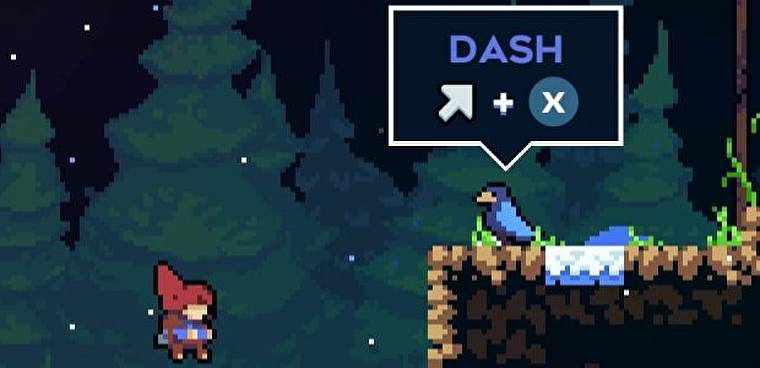
\includegraphics[width=7cm]{imgs/dash.jpeg}
\end{center}

\paragraph{Platformers are one of the common pitfalls for Indie Developers, but Celeste gets the \emph{feel} right, achieved by standing on the shoulders of Towerfall, developers' previous game which features some similar interactions.}

\section*{Story and Soundtrack}

\paragraph{Celeste is way more than what it seems at first glance. It does a great job portraying depression and anxiety in a way only the video game media can do through its story, soundtrack and gameplay.}

\section*{Final Thoughts}

\paragraph{Celeste is indeed an unique game and a good demonstration of what this media can achieve.}

\end{document}